\chapter{Problem Identification}
\begin{spacing}{1.0}
\setlength{\parskip}{0.3in}
\graphicspath{{./Chapter1/}}

\section{Introduction}
Beximco Communications Limited is a joint venture between Beximco Holdings Limited and General Satellite Group AG. Beximco Communications Limited has a core brand which is AKASH DTH. For Bangladeshi viewers AKASH DTH offers the world-class television watching experience through its Direct to Home (DTH) satellite TV service. AKASH DTH is the first DTH service in Bangladesh which is a method of receiving television signals directly from the satellite. AKASH DTH provides the best quality of picture and stereo sound. The satellite beam AKASH DTHsatellite ABS 2 is directly on our country that delivers the best digital TV service and HD channels to all the AKASH DTH subscribers. AKASH DTH aims to provide best DTH plans, Flexible DTH offer and packages and variation of digital internationals and local digital channels ranging from entertainment, sports, music to news and documentaries to their customers. To enjoy this hassle-free service and digital TV viewing experience customers have to connect the Set Top Box (STB) to a fixed satellite dish on the roof. With AKASH DTH the days of analogue cable are gone and as it offers all to experience the best DTH service in Bangladesh. With AKASH DTH TV viewing experience gets in a whole new level by not only digital channels but also HD picture quality. AKASH DTH provides its service across the country as it’s signal is available nationwide. Moreover, currently AKASH DTH runs its business in six core parts of the country like Dhaka, Chittagong, Sylhet, Rajshahi, Rangpur and Khulna.
\subsection{What is DTH service}
Direct to Home (DTH) also known as Direct Broadcast Satellite (DBS) is a method of receiving satellite television by means of signals transmitted from direct broadcast satellite. All the major services including DirecTV, Dish Network, Bell TV, Shaw Direct, and Sky use direct-broadcast satellites. DTH service ensures high picture quality and stereo sound as the signals are transmitted using Ku band.
Before DTH service was introduced signals were sent from fixed service satellites on the C band analog and received with only systems, which had more disadvantages to DTH service including the requirement of large satellite dishes and cable infrastructure. Moreover, it is not possible to reach everywhere with cable. In remote areas like hill tracks cable network is unavailable or very poor. For most of them TV is the only source of entertainment. They need better entertainment in their life which DTH service can fulfill. Whereas Cable TV is through cable networks, DTH service is wireless. Consumers can enjoy this service through a personal dish and a set-top box. DTH service is already popular in our neighboring countries. It has more advantages to cable network .In cable network after receiving the signal the signal is distributed through cable which causes signal loss. The more the distance the more signal loss occurs, thus the picture quality is compromised.
\subsection{How does AKASH DTH service work}
DTH stands for Direct to Home; as the name says, consumers will receive a signal directly from the satellite through the dish installed at their premise. In order to access the AKASH service, users will need a set top box, dish and other equipment as recommended by the company. 
\subsection{Features provided by AKASH DTH}
AKASH has brought to use the first world standard DTH service in Bangladesh with crystal clear picture \& sound, professional installation \& after sales service, 24/7 active helpline \& lots of other features. AKASH will even work for 14 inch black \& white TV. AKASH is the purveyor of supreme quality picture \& sound.  AKASH provides the real HD quality picture \& sound. AKASH provides features like program guide up to 7 days, upon its availability, where users can see schedules \& details of all the programs of their subscribed channels, favorite channel listing, program reminder feature \& even parental control (a feature that gives users option to lock channels that they don't want their children to watch). Soon more features will be introduced. They are the first \& only one at this moment to provide such a world class service.
\subsection{Business Agreements}
\subsubsection{Strategic Partnership with Robi Axita Limited}
Robi Axiata Limited and Beximco Communications Limited have recently signed a strategic partnership agreement. This agreement has paved the way for both the companies to collaborate for the promotion of Beximco Communications recently launched flagship DTH brand, AKASH.
\subsubsection{Agreement with OK wallet}
OK Wallet users get the facility to pay the bill for AKASH DTH with a cash back offer. AKASH DTH, the country's first ever DTH service, has signed an agreement with ‘OK Wallet’, the mobile financing service (MFS) of One Bank Limited. Under the agreement, OK Wallet users will enjoy two hundred taka cashbacks from AKASH DTH while getting a connection and can pay DTH bills easily with this wallet account. The regular price of the connection is BDT 5,499.
\subsubsection{Agreement with BCSCL}
Bangladesh Communication Satellite Company Limited (BCSCL) and Beximco Communications Limited (BCL) has signed two separate commercial agreement on Satellite Transponder Service and Up-linking Service respectively.Under the agreements, Beximco Communications will provide country’s first ever DTH service with brand name AKASH through the very first satellite of the nation- Bangabandhu Satellite The agreements were signed at an event held in BCSCL head office in the capital Dhaka on July 29, 2019.
\subsubsection{MoU with Evaly}
AKASH and the e-commerce marketplace Evaly have signed an agreement. Under the agreement, customers can now purchase Akash's connectivity services from Evaly. DS Faisal Hyder, Chief Executive Officer (CEO) of Beximco Communications Ltd and Evaly Chairman Shamima Nasrin signed the agreement on behalf of their respective organizations at a hotel in the capital yesterday on January 12, 2021.
\subsection{Channels and Packages}
Right now AKASH DTH has two packages- AKASH Standard at BDT 399 monthly and AKASH Lite at 249 monthly. In addition to AKASH Lite Package, 4 add on packs are introduced to offer subscribers the freedom of choice. Consumers can design their package as they like.
They have 120 channels including relevant \& popular Bangladeshi and foreign ones. 
Right now AKASH DTH is offering 75+ Standard Definition (SD) \& 40+ High Definition (HD) channels; Their HD channel can deliver true quality of HD which is not possible for regular cable connection. Cable isn't technologically capable of providing true 1080p HD view. 

\subsection{Management Hierarchy}
\begin{figure}[H]
	\centering
	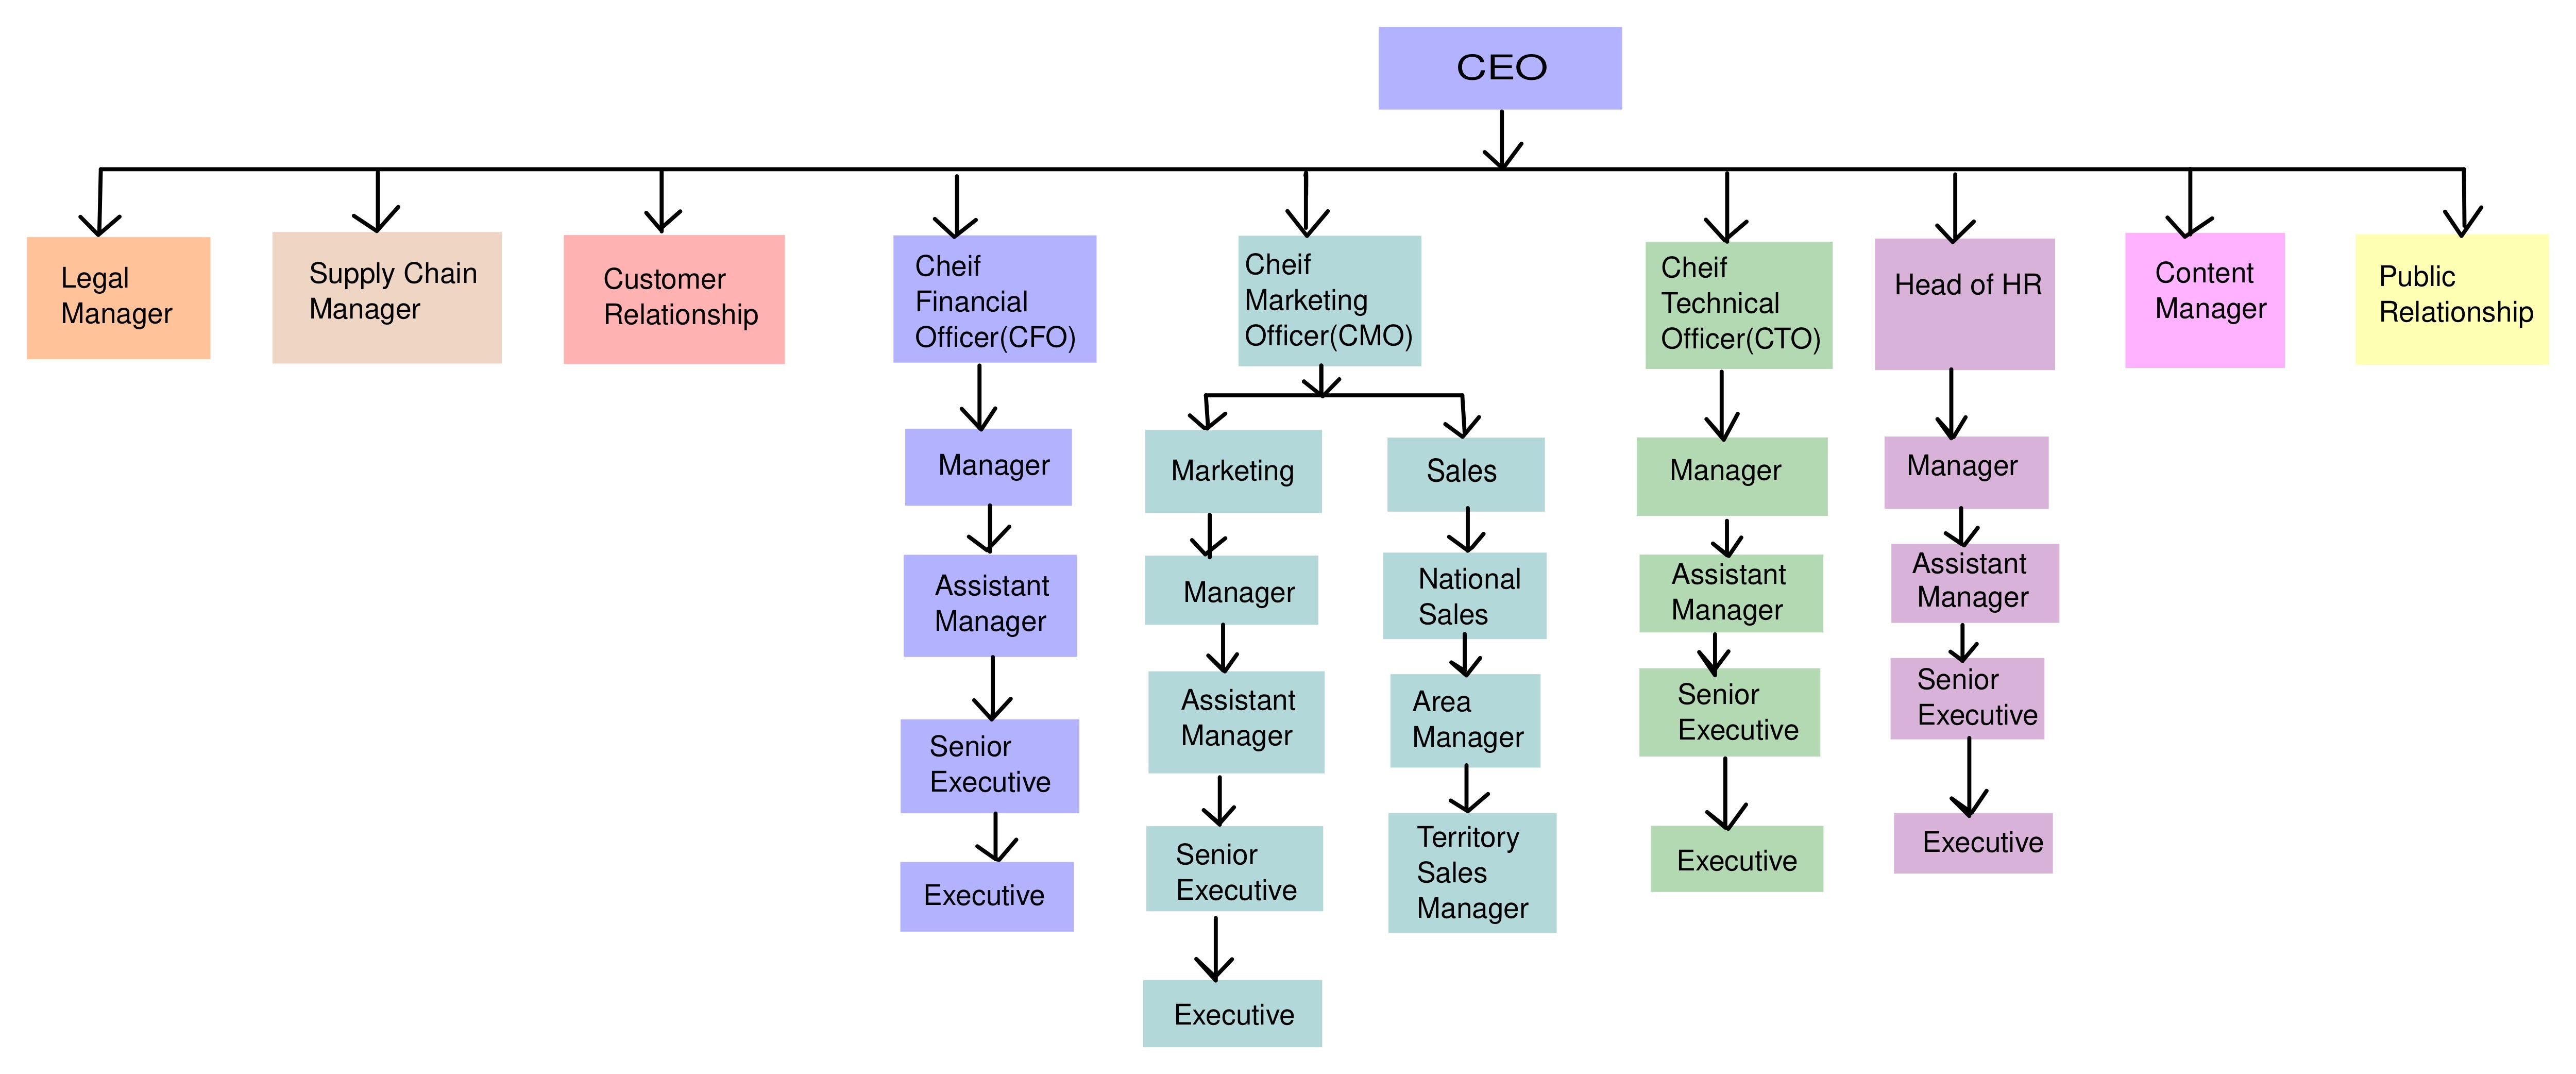
\includegraphics[width=\textwidth]{hierarchy}
	\caption{Management Role Hierarchy}
	\label{fig:hierarchy}
\end{figure}

\section{Problem Identification}
Though AKASH DTH is committed to deliver the best service in the country, there are some problems in user end. The major problems are:
\begin{enumerate}

\item Bad weather and signal problem
\item Pricing issue
\item Lack of some popular channels
\item Hardware related issues

\end{enumerate}

\section{Conclusion}
To analysis and design an information system for any organization, study their working methodology, management system and business policies is the first step. Identifying the problems and limitations of the existing system is the basis for further improvement of that system. In the initial phase, we studied about the targeting system of Akash DTH and identified some primary problems to their existing systems.     
\end{spacing}

\newpage
